% Template for MEng/BEng/MSc final reports
% EEE Department - Imperial College London
%
% INSTRUCTIONS
% (1) Compile using LuaLatex (it is the successor of pdflatex). To check this on Overleaf, click on the Menu on the top left.
% (2) Complete the SETUP below
% (3) Students of Imperial College can claim a free premium Overleaf account, see https://www.imperial.ac.uk/admin-services/ict/self-service/computers-printing/devices-and-software/get-software/get-software-for-students/overleaf/ 
% Claim the free premium account because as your report becomes more and more complex you may reach the timeout limit of the free account.

%%%%%%%%%%%%%%%%%%%%%%%%%%%%%%%%%%%%%%%
% DO NOT MODIFY FROM HERE ...
\documentclass[10pt]{ic_eee_thesis}

\usepackage[style=ieee,backend=biber,hyperref=auto]{biblatex}
\addbibresource{references.bib}
% ... TO HERE
%%%%%%%%%%%%%%%%%%%%%%%%%%%%%%%%%%%%%%%


%%%%%%%%%%%%%%%% SETUP %%%%%%%%%%%%%%%%
%%%%%%%%%%%%%%%%%%%%%%%%%%%%%%%%%%%%%%%
% EDIT THE FOLLOWING INFORMATION WITH YOUR DATA
% COMPLETE PART A
% IF YOU ARE DOING A MENG/BENG COMPLETE ALSO PART B
% IF YOU ARE DOING AN MSC IGNORE PART B
% LINES STARTING WITH % ARE COMMENTS. UNCOMMENT JUST ONE OF A SET OF OPTIONS
% MAKE SURE YOU CHECK AND UPDATE ALL INFORMATION, INCLUDING SUBMITYEAR


%%%%%%%%%%% PART A %%%%%%%%%%%
% PICK A DEGREE FROM THE LIST BELOW 
% BY COMMENTING OUT/IN YOUR DEGREE
% DO NOT MODIFY THE NAMES
%\degree{MEng}
%\degree{BEng}

\degree{MSc}

\title{Participatory Decision‑Making via a Discord Governance Bot}
\subtitle{A Computational Social Choice Approach} % use \subtitle{} to remove the subtitle
\author{Vedant Vasu Gupta}
\cid{06010159}
\supervisor{Dr\   Jeremy Pitt and Ciske Smit} %UK: Dr no dot, prof has dot
\submityear{2025}

% PICK A COURSE FROM THE LIST BELOW 
% DO NOT MODIFY THE NAMES
%%%%%%%%% BENG-MENG COMMON LIST
%\course{Electrical and Electronic Engineering}
%\course{Electronic and Information Engineering}
%%%%%%%%% MENG-ONLY LIST
%\course{Electrical and Electronic Engineering with Management} 
%\course{Electrical and Electronic Engineering with a Year Abroad}
%\course{Electronic and Information Engineering with a Year Abroad}
%%%%%%%%% MSC LIST
%\course{Analogue and Digital Integrated Circuit Design}
\course{Applied Machine Learning}
%\course{Communications and Signal Processing}
% \course{Control and Optimisation}
%\course{Future Power Networks}


% Do you want a list of figures?
% Do you want a list of tables?
% Do you want an acknowledgement page?
% Do you want a list of acronyms?
\setboolean{list_of_figures}{true} % false or true - Default is true
\setboolean{list_of_tables}{false} % false or true - Default is false
\setboolean{acknowledgement}{true} % false or true - Default is true
\setboolean{acronyms}{true} % false or true - Default is true

% If you want to print your thesis, consider changing the command below to true. If true, the command adds labels at the edge of the pages which will make easy to identify a chapter running through the pages with the finger. It is just a visual setting. The default values are different for MENG/BEng and MSc as a consequence of the different approval process. In any case, you can change this to either true or false as you prefer.
%\setboolean{edge_labels}{false} % default for MEng
\setboolean{edge_labels}{true} % default for MSc

%The preferred spacing for FYP/MSc reports is doublespacing. This is because it is easier for markers to annotate the document while marking. Some students requested the implementation of the singlespacing option. This can be activated below by changing from true to false, but discuss this with your supervisor first.
\setboolean{double_spacing}{true} %Default is true. If you want to change this, ask your supervisor if they are OK with singlespacing.

%%%%%%%%%%% PART B %%%%%%%%%%% 
% ONLY FOR MENG/BENG. MSC IGNORE THIS
% THESE ADDITIONAL SETTINGS HAVE BEEN ASKED BY THE MEng COMMITTEE BUT NOT BY THE MSC COMMITTEE
% Is this an interim report or final thesis?
\setboolean{final_thesis}{true} % true for final Thesis / false for interim report
\secondmarker{Second Marker\\[2mm]{\large \textsc Dr Jane Doe}} %If you do not know who your second marker is, use \secondmarker{}

%%%%%%%%%%%%% END SETUP %%%%%%%%%%%%%%%
%%%%%%%%%%%%%%%%%%%%%%%%%%%%%%%%%%%%%%%


% ADDITIONAL PACKAGES
% You can add your packages below. Note that the following packages are already loaded: pgfcore, geometry, bookmark, graphicx, setspace, kantlipsum, fontspec, polygrossia (default English), minitoc, silence, background, xpatch, tikzpagenodes, totcount, fancyhdr, titlesec and the tikz libraries calc, shapes.symbols and shapes.misc  

%Examples
\usepackage{amsmath}
\usepackage{amsfonts}
\usepackage{booktabs} % for professional tables
\usepackage{algorithm}
\usepackage{algpseudocode}
%...
\usepackage{acronym} % for acronym support
% ADDITIONAL COMMANDS
%Examples
\DeclareMathOperator{\diag}{diag}
\DeclareMathOperator{\vect}{vec}
%...


\begin{document}

\preamble % Do not change - required

% EDIT THE CONTENT OF THE FILES
% Abstract.tex
% OrigSta_Copyright.tex
% Acknowledgement.tex
% You can find them under the folder 
% "chapters" on the left column

% ADD AS MANY CHAPTERS AS NEEDED
% BY CREATING .TEX FILES IN THE FOLDER chapters
% AND ADDING \input{namechapter.tex} BELOW
% Chapter ordering: introduction, literature review, design methodology,
% implementation details, experiments and results, discussion, and reflections.
\doublespacing % Do not change - required

\chapter{Introduction}
\label{ch:introduction}

%%%%%%%%%%%%%%%%%%%%%%%%%%%%%%%%%%%%%%%
% IMPORTANT
\begin{spacing}{1} %THESE FOUR
\minitoc % LINES MUST APPEAR IN
\end{spacing} % EVERY
\thesisspacing % CHAPTER
% COPY THEM IN ANY NEW CHAPTER
%%%%%%%%%%%%%%%%%%%%%%%%%%%%%%%%%%%%%%%

\section{Background and Motivation}

Collective decision‐making is a fundamental activity of human societies.  When
groups must choose a policy, allocate resources or establish a social norm, they
need to aggregate diverse preferences into a single outcome.  The field of
\emph{social choice theory} formalises this problem and studies the properties of
different aggregation mechanisms.  Arrow’s impossibility theorem famously
showed that no rank‑ordering rule can simultaneously satisfy four key axioms—unrestricted domain, Pareto
efficiency, independence of irrelevant alternatives, and non‑dictatorship \cite{Arrow1951}.  Subsequent theorists have
argued that the real problem of social choice is to determine which
combination of gains and losses across individuals is socially
preferable \cite{Black1958, Okasha2011}.  These results highlight fundamental
trade‑offs between fairness, representativeness and manipulability.

With the proliferation of online communities on platforms such as Discord and
Slack, collective decision‑making increasingly occurs through digital
interfaces.  However, the native polling tools offered by these platforms are
rudimentary: they typically limit the number of options, do not allow ranked or
weighted voting, and provide little transparency about how winners are
determined.  Communities therefore require governance tools that embed richer
voting mechanisms while remaining accessible to non‑experts.

Recent work in socio‑technical systems argues that legitimate governance
requires continuous civic participation across the \emph{engage–envision–enact}
cycle.  Mertzani \emph{et~al.} \cite{Mertzani2023Engage} note that democracy should not be treated as a
static, universally optimal regime; anthropological and political evidence
demonstrates that democratic institutions evolve and may require adaptation to
remain fit for purpose.  They argue that legitimate
consent arises when governance processes are meaningful, informed and
revocable, and that communities must be empowered to reflect on and
reconfigure their social arrangements.  Related research on socially‑guided
machine learning emphasises that hybrid human–AI systems risk reinforcing
existing power asymmetries unless those affected participate in designing and
modifying decision mechanisms \cite{Mertzani2025SGML}.  Together, these
perspectives motivate the design of participatory governance tools that
encourage reflection, support multiple voting methods and respect user
autonomy.

\paragraph{Limitations of native polls.}  The standard polling
widgets provided by Discord and similar platforms present only a small
 number of options and permit users to select, at most, one.  They
implement a simple plurality rule whereby the alternative with the
largest number of votes wins; no majority is required, and ties are
handled arbitrarily \cite{Black1958}.  Such rules ignore the intensity of
preferences and cannot accommodate ranked or weighted ballots.  In
 addition, the User Interface (UI) does not allow participants to express
indifference or approval for multiple options.  From a theoretical
 perspective, these limitations map directly to the impossibility
results of social choice: Arrow’s theorem shows that no ranked‑choice
rule can simultaneously satisfy fairness criteria such as the
independence of irrelevant alternatives and non‑dictatorship; all
rules entail trade‑offs \cite{Arrow1951}.  By restricting
choice to a single checkbox, native polls implicitly select one point
in this trade‑off space without giving communities the ability to
choose alternative mechanisms.  Our motivation is therefore to
construct a platform that exposes multiple voting rules, supports
the expression of preferences through ranking and weighting, and remains usable for
non‑experts despite the constraints of the Discord interface.

\section{Objectives}

The overarching research question of this thesis is:

\begin{quote}
\emph{How can an online governance tool support diverse and expressive voting mechanisms while remaining usable and trustworthy to community members?}
\end{quote}

To address this question, we pursue four objectives:
\begin{enumerate}
    \item \textbf{Theoretical review}: Survey the foundations of social choice
    theory, PD and algorithmic governance, emphasising the
    trade‑offs uncovered in the literature.
    \item \textbf{System design}: Formally specify and implement a
    governance tool integrated within the chat platform that enables proposal submission and
    supports multiple voting mechanisms—plurality, Borda, approval,
    instant runoff and Condorcet—together with an optional weighted
    scheme.  The design emphasises a clear architecture with
    well‑defined components, data models and algorithms rather than a
    chronological narrative of software development.  All interface
    elements must respect the platform’s limitations on modals and
    components while remaining intuitive for non‑expert users.
    \item \textbf{Empirical evaluation}: Design and conduct a controlled
    experiment using a \emph{Day~Out} scenario.  Ten participants took
    part in both plurality and weighted voting sessions and completed pre‑ and
    post‑surveys measuring their satisfaction with the process and outcome, perceptions of fairness and the extent to which the final decision reflected the group’s preferences, as well as their willingness to reuse the mechanism.  The resulting data are analysed in Chapter~\ref{ch:experiments}, where we report descriptive statistics, compare the two voting methods and summarise participants’ preferences and qualitative feedback.
    \item \textbf{Reflection and impact}: Reflect on the strengths and
    limitations of the system, propose future improvements—including a
    machine‑learning–based \emph{what‑if} predictor—and assess the
    environmental and societal impacts of participatory governance.
\end{enumerate}

\section{Structure of the Thesis}

The remainder of the thesis is organised as follows.  Chapter~\ref{ch:litreview}
presents a literature review of social choice theory, participatory and
power‑sensitive design, digital voting systems and fairness criteria.
Chapter~\ref{ch:method} introduces the methodology and high‑level system
design, presenting the guiding principles and architecture of the governance
tool.  Chapter~\ref{ch:implementation} details the technical implementation,
describing the components, data model, algorithms and user‑interface flows.
Chapter~\ref{ch:experiments} describes the experimental setup, reports the collected data and compares the plurality and weighted voting conditions.
Chapter~\ref{ch:discussion} interprets the results, situates them within
the broader literature and critiques the system’s strengths and limitations.
Chapter~\ref{chLast} contains reflections on legal, ethical, environmental
and inclusion aspects of the work, together with project limitations and
technical challenges.  Finally, Chapter~\ref{ch:conclusions} concludes the
thesis and outlines directions for future research.
\doublespacing % Do not change - required

\chapter{Literature Review}
\label{ch:litreview}

%%%%%%%%%%%%%%%%%%%%%%%%%%%%%%%%%%%%%%%
% IMPORTANT
\begin{spacing}{1} %THESE FOUR
\minitoc % LINES MUST APPEAR IN
\end{spacing} % EVERY
\thesisspacing % CHAPTER
% COPY THEM IN ANY NEW CHAPTER
%%%%%%%%%%%%%%%%%%%%%%%%%%%%%%%%%%%%%%%

This chapter synthesises the theoretical and empirical foundations
underpinning the design of our participatory governance bot.  We first
survey key results from social choice theory and introduce the voting
methods implemented in the system.  We then review existing digital
voting systems that operate within constrained UIs, drawing
lessons from the design patterns and limitations of popular tools on
Discord and Slack.  Next we discuss Participatory Design (PD) principles for
collaborative decision tools, followed by a review of research on
user‑experience (UX) and cognitive considerations for voting
interfaces.  Finally, we summarise computational considerations and
fairness criteria that guide our later analysis of the implemented
mechanisms.

\section{Foundations in Social Choice Theory and Voting Methods}

Social choice theory studies how individual preferences can be aggregated
into a collective decision.  A \emph{voting rule} takes as input a set of
alternatives and the voters’ preference orderings and outputs either a
winner or a social ordering.  Arrow’s impossibility theorem shows that
no rank‑ordering rule on three or more alternatives can simultaneously
satisfy unrestricted domain, Pareto efficiency, independence of
irrelevant alternatives and non‑dictatorship \cite{Arrow1951,Gibbard1973,Satterthwaite1975}.
This negative result forces any voting rule to compromise on at least
one desirable property.  Gibbard and Satterthwaite further showed that
with at least three alternatives any non‑dictatorial deterministic rule
that always selects a winner is susceptible to strategic
manipulation; there is no strategy‑proof rule other than random
dictatorship for unrestricted preferences.  These impossibility results
motivate the plurality of voting methods used in practice and
implemented in our system.

\subsection{Positional and Approval Rules}

\emph{Positional scoring rules} assign points based on an option’s
position in each voter’s ranking.  The simplest is the plurality rule:
only the top‑ranked option on each ballot earns a point, and the option
with the largest first‑place count wins \cite{Black1958}.  The Borda
count assigns each option a number of points equal to the number of
options ranked below it; summing these scores yields a winner \cite{Borda1784}.  Approval voting discards rankings entirely: voters
mark any number of options they approve, and the option with the most
approvals wins \cite{Black1958}.  These rules are computationally
simple (polynomial time) and satisfy anonymity and neutrality, but they
violate other criteria such as the independence of irrelevant alternatives
or the Condorcet criterion.

\subsection{Runoff and Pairwise Methods}

Runoff methods simulate a series of rounds.  Instant‑runoff voting
(also known as the single transferable vote) repeatedly eliminates the
option with the fewest first‑place votes and redistributes those votes
according to the next preferences until a single option remains \cite{Bartholdi1989}.
Condorcet methods compare options pairwise: an option that defeats every
other option in head‑to‑head comparisons is the Condorcet winner and
should be elected \cite{Condorcet1785}.  In the absence of a Condorcet
winner, methods such as the Schulze or ranked pairs rule select a
winner by constructing a ranking that respects as many pairwise
preferences as possible.  Computing an exact Kemeny ranking—which
maximises the number of pairwise agreements—is NP‑hard, illustrating
that some desirable rules are computationally intractable.  Our bot
implements plurality, Borda, approval, instant runoff and Condorcet
counting in a modular fashion and avoids NP‑hard methods in favour of
polynomial‑time algorithms.

\subsection{Cardinal and Weighted Mechanisms}

Cardinal mechanisms allow voters to express intensities rather than
just orderings.  Quadratic voting endows each participant with a budget
of voice credits; buying $v$ votes costs $v^2$ credits, making
additional votes progressively more expensive \cite{Bartholdi1989}.
Such mechanisms can reveal how strongly individuals feel about
alternatives but may favour participants with larger budgets.  Our
implementation uses a simplified weighted approach: each voter receives
a fixed endowment of tokens and allocates them across alternatives.
Token allocations are summed to compute weighted scores, balancing
expressiveness with equity.  The design acknowledges the normative
debates around cardinal voting and retains anonymity by assigning
equal budgets to all participants.

\section{Digital Voting Systems in Constrained UIs}

Beyond theoretical considerations, practical implementations of digital
voting systems must operate within the constraints of chat platforms.
Discord and Slack are popular environments for community governance, but
their interfaces offer limited interaction primitives—typically
commands, reactions, buttons and modal dialogs.  Existing bots tend
to implement only simple voting rules.  For example, the Votex bot
allows administrators to assign a multiplier to each role; votes are
weighted accordingly, enabling DAOs and councils to run weighted polls
using a slash command \cite{ZikenLabs2024}.  Dyno and EasyPoll are
general‑purpose moderation bots that provide a \texttt{?poll} command,
adding reaction emojis for each option and counting the reactions after
an expiration period.  Such reaction‑based polls use plurality
exclusively and provide no support for ranked or weighted voting.  On
Slack, the Polly.ai application simplifies real‑time feedback by letting users run
polls and surveys directly in chat; it is best known for facilitating
on‑the‑fly questions and quizzes and presenting results instantly in the
chat interface \cite{ZapierSlackPoll2023}.  Despite their popularity,
these tools share limitations: they restrict users to binary or
unordered inputs, provide little control over anonymity or timing and
lack extensibility for experimenting with alternative rules.

These observations motivate the design of a more expressive governance
bot.  Our implementation leverages Discord’s limited UI primitives to
support multiple voting rules, ranking, and weighted token allocation
without requiring external websites.  The challenges of constrained
interfaces are revisited in Chapter~\ref{ch:implementation} when
describing the UI flows.

\section{Participatory Design in Collaborative Decision Tools}

PD emphasises involving stakeholders throughout
    the development process so that technology reflects their values,
requirements and constraints \cite{Schuler1993,Schneider2018}.  Value‑sensitive design (VSD) extends PD
by making explicit the values—such as democracy, privacy and fairness—
that are embedded in artefacts.  Power‑sensitive design (PSD) further
acknowledges that socio‑technical systems can reproduce or amplify
existing power asymmetries.  Mertzani \emph{et~al.} advocate an
\emph{engage–envision–enact} cycle: communities should continuously
engage in governance, envision alternative regimes and enact changes
in response to shifting circumstances.  They caution against treating
democracy as an immutable ideal and highlight how governance practices
vary across cultures and contexts.  In the socially‑guided machine
learning framework, hybrid human–AI systems are co‑designed to empower
communities while preserving equity and transparency.  These principles
inform the design requirements of our bot: user control, extensibility
and accessibility.  Stakeholders must be able to choose voting rules,
adjust token budgets and override decisions; the software must be
modular and open to modification; and the interface should lower
barriers to participation for novices.

\section{UX and Cognitive Aspects of Voting Interfaces}

Voting interfaces must balance expressiveness—the ability to capture
complex preferences—and usability, which demands simplicity to reduce
cognitive load.  Presenting a long list of options in a single form may
overwhelm users, leading to abandonment or heuristic shortcuts.  Ranked
ballots require voters to articulate an order for every alternative,
which can be cognitively taxing when many options exist.  Cardinal mechanisms add another layer of complexity by asking users to allocate
limited budgets.  To mitigate these issues, designers can break tasks
into smaller steps, provide progress indicators and limit the number of
options displayed at once.  Empirical work comparing chatbot and menu‑based
interfaces shows that cognitive load and user satisfaction depend strongly on the simplicity of interaction \cite{Nguyen2022}.  Another concern is the \emph{bandwagon
effect}: when interim results are visible, voters may follow the
majority rather than expressing independent preferences.  Hiding
intermediate tallies until voting closes can reduce this bias.  Our
bot adopts these UX principles: ranking and token allocation are
elicited through sequential dialogs with clear feedback; progress bars
indicate how many tokens remain; and voting results are hidden until
the deadline.  These choices are grounded in cognitive psychology and
relevant literature on digital polling interfaces \cite{[ADD CITATION for cognitive psychology in digital polling interfaces]}.

\section{Computational Considerations and Fairness Criteria}

Implementing voting rules requires balancing computational
tractability with normative desiderata. \cite{[ADD CITATION for trade-offs in computational social choice]}  Some rules, such as plurality,
Borda and approval, can be computed in linear time in the number of
votes.  Instant‑runoff and Condorcet methods require sorting and pairwise
comparison but remain polynomial‑time.  Kemeny ranking, in contrast, is
NP‑hard; our system avoids it to ensure scalability.  Beyond complexity,
fairness axioms help evaluate and compare rules.  \emph{Anonymity}
requires that outcomes depend only on the multiset of ballots, not on
voter identities.  \emph{Neutrality} demands that all alternatives are
treated symmetrically.  The \emph{majority criterion} states that if
some alternative is ranked first by a majority of voters, it should win.
The \emph{Condorcet criterion} requires that a Condorcet winner, if it
exists, must be elected.  \emph{Monotonicity} holds that raising an
option’s position in any ballot should not harm its chances.  No single
rule satisfies all criteria simultaneously—an echo of Arrow’s theorem.
In later chapters we use these criteria to reflect on the strengths and
limitations of the implemented voting mechanisms.

\doublespacing % Do not change - required

\chapter{Methodology and System Design}
\label{ch:method}

%%%%%%%%%%%%%%%%%%%%%%%%%%%%%%%%%%%%%%%
% IMPORTANT
\begin{spacing}{1} %THESE FOUR
\minitoc % LINES MUST APPEAR IN
\end{spacing} % EVERY
\thesisspacing % CHAPTER
% COPY THEM IN ANY NEW CHAPTER
%%%%%%%%%%%%%%%%%%%%%%%%%%%%%%%%%%%%%%%

This chapter formalises the methodology used to design and implement the
participatory governance bot.  We specify the final system from the perspective of computer science: the requirements and design
principles that informed it, its high‑level architecture, the roles of
its components, the underlying data model, the core algorithms that
compute outcomes and the UI flows that elicit and record
preferences.   

\section{System Requirements and Design Principles}

The bot was developed according to three guiding principles that also
constitute system requirements.  Each principle reflects a normative
criterion derived from participatory and power‑sensitive design and
translates into concrete software features:

\begin{enumerate}
    \item \textbf{Accessibility and Inclusivity}.  The interface must be
    intuitive and accessible to users regardless of their technical
    expertise.  In practice this requirement led to the adoption of
    simple button‑based views rather than text commands.  For example,
    the proposal creation workflow in \texttt{proposals.py} uses a
    \texttt{discord.ui.Modal} to solicit a title and description from
    the user, and presents a button menu for selecting the voting
    mechanism.  The voting views in \texttt{voting.py} display one
    question at a time and provide clear instructions and progress
    indicators.  Input validation and informative error messages
    minimise cognitive load and encourage broad participation.
    \item \textbf{User Control and Revocability}.  Participants retain
    agency throughout the governance process.  They can propose
    alternatives, choose among supported voting rules, allocate tokens within their budget and withdraw consent at any
    time.  Commands in \texttt{main.py} are explicitly invoked by
    users; the bot never autonomously initiates decisions or allocates
    tokens.  This design adheres to the Engage–Envision–Enact
    principle of meaningful, informed and revocable participation
    \cite{Mertzani2023Engage}.  The ability to choose a voting rule
    empowers communities to experiment with different social choice
    functions and to explore trade‑offs between expressiveness and
    simplicity.
    \item \textbf{Extensibility and Maintainability}.  The system must
    accommodate new voting mechanisms, user roles and data collection
    features without extensive refactoring.  To achieve this, the
    architecture separates responsibilities into modules: the
    persistence layer in \texttt{db.py}, the UI in
    \texttt{proposals.py} and \texttt{voting.py}, the counting
    algorithms in \texttt{voting\_utils.py} and the orchestration and
    background tasks in \texttt{main.py}.  Each module exposes
    asynchronous functions that encapsulate their state and avoid
    blocking the event loop.  Adding a new voting rule amounts to
    implementing a new counting function and associated view without
    modifying the existing infrastructure.  This modularity also
    facilitates testing and integration with alternative platforms in
    the future.
\end{enumerate}

\section{High‑Level System Architecture}
The bot is implemented in Python using the asynchronous
\texttt{discord.py} library and adheres to an event‑driven architecture.
When the bot connects to a server it registers event handlers for
commands (such as proposal submission and vote casting) and user
interactions (button clicks or modal submissions).  These handlers
enqueue tasks into an \texttt{asyncio.Queue}; a background worker
processes the queue to update tracking messages and publish results.
The architecture is decomposed into five cooperating subsystems:
\begin{itemize}
    \item \textbf{Discord API}.  The remote service delivers
    messages, button presses and modal submissions to the bot and
    conveys the bot’s responses back to users.  The bot must respect
    API rate limits and handle network failures gracefully.
    \item \textbf{Bot core (\texttt{main.py})}.  This entry point
    instantiates the Discord client, registers event handlers, schedules
    background tasks to check proposal deadlines and to announce
    results, and mediates between the UI and the logic
    layer.  It maintains an \texttt{asyncio.Queue} to decouple
    asynchronous updates from user interactions and provides utility
    commands for administrators to inspect and modify settings.
    \item \textbf{UI components (\texttt{proposals.py} and
    \texttt{voting.py})}.  These modules implement the interactive
    workflows for proposal creation, campaign setup and voting.  They
    construct modal dialogs (e.g., to gather a title, description and
    options) and button‑based views for selecting a voting rule,
    ranking alternatives, approving options or allocating tokens.
    \item \textbf{Logic and algorithms (\texttt{voting\_utils.py})}.
    This module encapsulates the voting rules and tallying procedures
    described in Section~\ref{sec:algorithms}.  It exposes pure
    functions that accept ballots and token allocations and return
    winners and rankings under both unweighted and weighted conditions.
    \item \textbf{Persistence layer (\texttt{db.py})}.  All
    proposals, options, votes, campaigns, user participation records
    and server‑level settings are stored in a SQLite database.  The
    module provides asynchronous functions for creating, querying and
    updating records while hiding SQL details from the rest of the
    system.
\end{itemize}


This decomposition ensures that changes in one component (such as
adding a new voting rule or a different persistence layer) do not
propagate unintended side effects to others.  Asynchronous programming
enables the bot to handle multiple concurrent interactions without
blocking the event loop, and the \texttt{asyncio.Queue} decouples
long‑running updates (such as posting result messages) from user
interactions.  The database schema is normalised to avoid redundancy
and to support efficient queries.

% ------------------------------------------------------------
% Implementation details have been moved to Chapter~\ref{ch:implementation}.
% This chapter focuses on high‑level design and methodological
% considerations.  The following section discusses computational and
% fairness considerations that informed the overall design.
\section{Computational Considerations and Fairness}
Having introduced the system requirements and the high‑level
architecture, we now discuss the computational and normative factors
that shaped the design.  A fundamental insight from social choice theory
is that no voting rule satisfies all fairness axioms simultaneously.
Arrow’s impossibility theorem shows that, for three or more
alternatives, no rank‑ordering rule can simultaneously satisfy
unrestricted domain, Pareto efficiency, independence of irrelevant
alternatives and non‑dictatorship \cite{Arrow1951}.  The Gibbard–Satterthwaite
theorem demonstrates that any deterministic, non‑dictatorial rule with at
least three alternatives is susceptible to strategic manipulation \cite{Gibbard1973,Satterthwaite1975}.  In
addition to these impossibility results, desirable axioms include:

\begin{itemize}
    \item \textbf{Anonymity} (all voters are treated equally);
    \item \textbf{Neutrality} (all alternatives are treated equally);
    \item \textbf{Majority criterion} (if a majority of voters rank an
    alternative first, that alternative should win);
    \item \textbf{Condorcet criterion} (if an alternative beats every
    other alternative in pairwise comparisons, it should win);
    \item \textbf{Monotonicity} (raising an alternative in a ranking
    should not hurt its chances of winning);
    \item \textbf{Participation} (no voter should benefit from abstaining).
\end{itemize}
Different rules satisfy different subsets of these axioms.  For
instance, plurality satisfies anonymity and neutrality but fails the
Condorcet criterion and majority criterion in some cases; Borda count
satisfies anonymity and neutrality but violates independence of irrelevant
alternatives; approval voting satisfies anonymity and neutrality and
reduces vote splitting but fails the Condorcet and majority criteria;
Condorcet methods satisfy the majority criterion and the Condorcet
criterion but may fail to produce a unique winner.  Weighted (token)
voting deliberately violates anonymity by design: voters allocate a
bounded budget of tokens to express intensity, trading off equality
against representational fairness.  Recognising these trade‑offs, our
approach empowers communities to choose among mechanisms according to
their priorities.

Computational complexity also constrains the choice of voting rules.
Many appealing rules are computationally intractable: computing the
Kemeny–Young consensus ranking—a method that seeks a ranking which minimises the number of pairwise disagreements with voters' preferences—is NP‑hard \cite{Bartholdi1989}, as is determining winners
under the Dodgson method.  To ensure responsiveness on a live Discord
platform, our bot implements only polynomial‑time rules: plurality,
Borda, approval, instant runoff and Condorcet (via simple pairwise
majority matrices).  This reflects the literature’s recommendation to
balance fairness with feasibility.  Future versions could explore
approximate algorithms or off‑loading heavy computations to external
services.

In summary, the methodology emphasises fairness, expressiveness and
computational tractability.  Detailed implementation of the components,
database schema, algorithms and UI flows are provided in
Chapter~\ref{ch:implementation}.  That chapter translates the
conceptual design presented here into concrete code.

% End of high-level methodology.  Detailed implementation sections have been
% removed from this chapter and now reside in Chapter~\ref{ch:implementation}.
\doublespacing % Do not change - required

\chapter{System Implementation}
\label{ch:implementation}

%%%%%%%%%%%%%%%%%%%%%%%%%%%%%%%%%%%%%%%
% IMPORTANT
\begin{spacing}{1} %THESE FOUR
\minitoc % LINES MUST APPEAR IN
\end{spacing} % EVERY
\thesisspacing % CHAPTER
% COPY THEM IN ANY NEW CHAPTER
%%%%%%%%%%%%%%%%%%%%%%%%%%%%%%%%%%%%%%%

This chapter details the technical implementation of the governance bot.
Where Chapter~\ref{ch:method} established the design principles and
high‑level architecture, here we describe how those concepts were
realised in code.  We document the roles of each software module, the
database schema, the algorithms used to tally ballots and the user
interaction flows.  Throughout the chapter we justify design choices
against the literature reviewed in Chapter~\ref{ch:litreview}.  For
example, the interface uses simple buttons and sequential prompts to
minimise cognitive load, in line with usability heuristics, and hides
interim tallies to mitigate the bandwagon effect.  The supported voting
rules are limited to those with polynomial‑time algorithms, reflecting
computational considerations discussed in the literature.

\section{Component Implementation}

Each module of the bot encapsulates a specific responsibility and
communicates with other modules via asynchronous function calls.  The
main components are as follows:

\paragraph{\texttt{main.py} (bot core).}  This file is the entry point
for the Discord client.  It registers command handlers for proposal
submission, voting initiation and administrative functions, and it
schedules background tasks such as \emph{deadline checks} and
\emph{result announcements}.  It maintains an \texttt{asyncio.Queue}
that acts as a task buffer.  When a vote is recorded or a proposal’s
status changes, messages are pushed onto the queue; a worker coroutine
consumes tasks to update tracking embeds or to post final results.  The
bot core also exposes commands for administrators to view and modify
server‑level settings (e.g., default voting mechanism and token
budget).

\begin{algorithm}
    \caption{Queue worker for vote tracking}\label{alg:queue_worker}
    \begin{algorithmic}[1]
        \Procedure{UpdateTrackingWorker}{bot, queue}
            \State Wait until \texttt{bot} is ready
            \While{\texttt{bot} is running}
                \State item $\leftarrow$ dequeue from \texttt{queue}
                \State Extract $guild\_id$ and $proposal\_id$
                \If{either identifier missing}
                    \State Log warning; mark task done; \textbf{continue}
                \EndIf
                \State guild $\leftarrow$ bot lookup of $guild\_id$
                \If{guild exists}
                    \State \Call{UpdateVoteTracking}{guild, $proposal\_id$}
                \Else
                    \State Log warning about missing guild
                \EndIf
                \State Mark task done and sleep for 5~s
            \EndWhile
        \EndProcedure
    \end{algorithmic}
\end{algorithm}

\paragraph{\texttt{proposals.py} (proposal and campaign creation).}
This module defines classes derived from \texttt{discord.ui.Modal} and
\texttt{discord.ui.View} to present interactive forms to users.  When a
user invokes the proposal command, a modal prompts for a title,
description, deadline and set of options.  For weighted campaigns the
modal additionally asks for the number of tokens per voter and the
number of sub‑decisions (e.g., breakfast, transport, activity, dinner).
Upon submission the module validates inputs, writes the proposal and
options to the database and notifies moderators.  It also displays a
view allowing the creator to select a voting mechanism.  The modular
design of these classes means that adding a new field or workflow
involves subclassing and overriding callbacks rather than editing the
bot core.

\paragraph{\texttt{voting.py} (user interaction during voting).}
This module contains a family of \texttt{discord.ui.View} classes that
guide the user through casting a ballot.  For plurality and approval
rules, the view displays a row of buttons corresponding to options and
records the user’s selection or approvals.  For ranked voting
(Borda, instant runoff and Condorcet), the view presents successive
choices asking the voter to select their next most preferred option
until a complete ranking is built.  For weighted voting, the view
displays increment and decrement buttons next to each alternative and a
progress bar indicating how many tokens remain.  When the user
confirms their choices, the view calls into the database to record the
ballot and triggers an update on the task queue.  The design ensures
that all user input is solicited through clear, sequential interactions
despite Discord’s limitations on interface components.  Hiding interim
results prevents social influence and bandwagon effects as discussed in
the literature.

\begin{algorithm}
    \caption{DM voting workflow}\label{alg:dm_voting}
    \begin{algorithmic}[1]
        \Procedure{SendVotingDM}{member, proposal, options}
            \State $proposal\_id \leftarrow$ extract from proposal
            \If{$proposal\_id$ missing} \State \Return \textbf{False} \EndIf
            \State Parse voting mechanism and hyperparameters
            \If{proposal part of a campaign}
                \State Fetch campaign details and enrol voter
                \State Retrieve remaining tokens for member
            \EndIf
            \State Compose embed with proposal metadata, options and deadline
            \If{anonymous voting enabled}
                \State Attach unique identifier for voter
            \EndIf
            \State Instantiate view corresponding to mechanism
            \State Send DM with embed and view
            \State \Return \textbf{True}
        \EndProcedure
    \end{algorithmic}
\end{algorithm}

\paragraph{\texttt{voting\_utils.py} (core logic).}
This module implements the counting algorithms for each supported
mechanism.  It provides pure functions that accept a list of ballots
and, where appropriate, token allocations and return a ranking of
alternatives and the winning option.  Section~\ref{sec:algorithms}
formalises these algorithms.

\paragraph{\texttt{db.py} (persistence layer).}
The database module defines the schema and provides asynchronous
functions to create and query records.  It stores servers, users,
settings, proposals, proposal options, votes and campaigns in separate
tables.  The functions abstract away SQL and return Python objects,
thereby preventing SQL injection and facilitating unit testing.  User
identifiers are hashed before insertion to protect privacy, and
foreign‑key constraints ensure referential integrity.

\paragraph{\texttt{utils.py} and other helpers.}
Auxiliary functions for time formatting, parsing durations, generating
progress bars and performing moderation actions reside in small helper
modules.  These utilities separate peripheral concerns from the core
logic.

\section{Data Model}

The system stores all persistent state in a normalised SQLite
database.  Each table encapsulates a distinct concept, and foreign keys
encode relationships between them.  The main tables are summarised
below:

\begin{description}
    \item[servers] One record per Discord server using the bot.  Fields
    include a unique server identifier (primary key), the server name
    and configuration parameters such as the default voting mechanism,
    whether weighted campaigns are allowed and the token budget.  When
    the bot joins a new server, a corresponding entry is created.
    \item[users] One record per participating user.  The primary key is
    an internal integer identifier; a hashed version of the user’s
    Discord ID is stored instead of the raw identifier to preserve
    anonymity.  Additional columns capture opt‑in status for weighted
    campaigns and optional demographic data if collected via surveys.
    \item[proposals] Each proposal represents a decision that a
    community wishes to make.  Columns include the server ID, the
    proposer’s user ID, a title and description, a deadline timestamp,
    the selected voting mechanism, a status flag (draft, active or
    closed) and whether the proposal is part of a weighted campaign.
    \item[proposal\_options] For each proposal, this table lists the
    alternative options.  Each row stores the option text and a
    foreign key back to the parent proposal.  Composite primary keys
    ensure uniqueness within a proposal.
    \item[votes] Each row records a user’s ballot on a proposal.  For
    ranked and approval votes the ballot is stored as a JSON‑encoded
    array of option identifiers; for weighted voting the tokens
    invested in each option are stored.  Additional columns capture
    the time of submission and whether the voter abstained.  A unique
    constraint on (proposal ID, user ID) prevents duplicate voting.
    \item[campaigns] Weighted campaigns group together multiple
    proposals under a single token budget.  Fields include the
    campaign name, start and end times, the number of tokens per voter
    and the list of proposals involved.  A separate table
    \texttt{user\_campaign\_participation} records how many tokens
    each user has invested so far in a campaign.
\end{description}

Indices are added on foreign keys to accelerate joins.  All database
operations are asynchronous to avoid blocking the event loop.  Hashing
user identifiers and storing only aggregated results complies with
data‑protection regulations and reduces the risk of re‑identification.

\section{Core Algorithms}
\label{sec:algorithms}

This section formalises the voting rules implemented by
\texttt{voting\_utils.py}.  Let $A$ be the set of alternatives, with
\(|A|=n\), and let $V$ be the set of voters.  A ballot is either a
ranking of all alternatives, a set of approved alternatives or a
vector of token allocations.  In the weighted case each voter is
endowed with a fixed budget of tokens $B$; the sum of tokens they
allocate across alternatives must equal $B$.

\begin{algorithm}
    \caption{Tally orchestrator}\label{alg:tally_orchestrator}
    \begin{algorithmic}[1]
        \Procedure{CalculateResults}{$proposal\_id$}
            \State proposal $\leftarrow$ fetch proposal metadata
            \If{proposal missing} \State \Return \textbf{None} \EndIf
            \State votes $\leftarrow$ fetch all votes for proposal
            \State Separate abstentions from effective votes
            \State options $\leftarrow$ load from database or fallback
            \State mechanism $\leftarrow$ determine from proposal
            \State results $\leftarrow$ \Call{count\_votes}{mechanism, effective votes, options, hyperparameters}
            \State Annotate results with abstain counts, token totals and options used
            \State Derive final status based on winner or vote totals
            \State \Return results
        \EndProcedure
    \end{algorithmic}
\end{algorithm}

\paragraph{Plurality.}  Each voter selects a single favourite
alternative.  The tally function counts the number of first‑choice
votes received by each alternative,
\begin{equation}
    s(a) = \sum_{v \in V} \mathbf{1}\{\text{voter }v\text{ ranks }a\text{ first}\},
\end{equation}
where $\mathbf{1}$ is the indicator function.  The alternative(s)
with the largest score win; ties are broken by randomly selecting
among the tied alternatives.  This rule corresponds to the native
Discord poll and suffers from the spoiler effect because only the
top preference is recorded \cite{Black1958}.

\paragraph{Borda count.}  In the Borda rule each ranking is converted
into a point vector.  If voter $v$ ranks alternative $a$ in
position $r_{v}(a)$ (with 1 denoting most preferred), then the
score assigned to $a$ by $v$ is $n - r_{v}(a)$.  The total
score for each alternative is
\begin{equation}
    s(a) = \sum_{v \in V} (n - r_{v}(a)),
\end{equation}
and the alternative with the highest total wins.  The Borda count
captures more information than plurality by considering the entire
ranking and is resistant to some strategic voting, but it violates
independence of irrelevant alternatives \cite{Borda1784}.

\paragraph{Approval voting.}  Each voter approves of any number of
alternatives.  The tally function counts the number of approvals per
alternative,
\begin{equation}
    s(a) = \sum_{v \in V} \mathbf{1}\{a \in A_{v}^{\text{approved}}\},
\end{equation}
where $A_{v}^{\text{approved}}$ is the set of alternatives
approved by voter $v$.  The alternative(s) with the highest approval
score win.  Approval voting reduces vote splitting and allows voters
to express indifference between multiple acceptable options
\cite{Black1958}.

\paragraph{Instant runoff voting (IRV).}  Also known as ranked
choice voting, IRV simulates a series of runoff elections.  At each
round the alternative with the fewest first‑choice votes is eliminated
and its votes are transferred to the next preferred remaining
alternative on each ballot.  The process continues until a single
alternative remains.  Formally, let $A^{(k)}$ be the set of
candidates remaining in round $k$.  Compute scores
\(s^{(k)}(a) = \sum_{v \in V} \mathbf{1}\{\text{first choice of }v\text{ in }A^{(k)}\text{ is }a\}\).  Eliminate the alternative with the smallest
$s^{(k)}$; set $A^{(k+1)} = A^{(k)} \setminus \{\text{eliminated}\}$ and repeat.  IRV guarantees a majority winner if one exists and avoids
the no–show paradox but is vulnerable to non‑monotonicity
\cite{Bartholdi1989}.

\paragraph{Condorcet method.}  A Condorcet winner is an alternative
that defeats every other alternative in head‑to‑head majority
comparisons.  Construct the pairwise majority matrix $M$ where
$M_{a,b}$ is the number of voters who prefer $a$ over $b$.
If there exists an alternative $c$ such that $M_{c,b} > M_{b,c}$
for all $b \neq c$, then $c$ is the Condorcet winner and is
selected.  If no such alternative exists (i.e., the majority
preferences form a cycle), a Condorcet‑consistent method such as the
Schulze algorithm can be applied to compute a ranking.  Condorcet
methods respect the majority criterion and are highly expressive but
may not always produce a unique winner \cite{Condorcet1785}.

\paragraph{Weighted (token) voting.}  To capture intensity of
preferences, each voter is given a budget $B$ of tokens to distribute
among the alternatives.  Let $t_{v,a}$ denote the number of tokens
invested by voter $v$ in alternative $a$, with the constraint
$\sum_{a \in A} t_{v,a} = B$.  The weighted score of each
alternative is
\begin{equation}
    s(a) = \sum_{v \in V} t_{v,a}.
\end{equation}
The alternative with the highest token sum wins.  Weighted voting
generalises approval voting (each approval contributes one token) and
is related to quadratic voting in which the cost of casting multiple
votes increases quadratically with the number of votes.  Our design
fixes a linear cost in tokens to simplify the user experience and
allocates an equal budget to each voter to preserve fairness.

In all rules ties are broken by either drawing at random among tied
alternatives or by applying a deterministic tie‑breaking rule (e.g.,
lexicographic order).  When run within a weighted campaign, the raw
vote counts and token sums are also recorded for post‑hoc analysis of
participation and investment behaviour.

\section{UI and Interaction Flow}

User interactions with the governance bot unfold along a small number of
well‑defined pathways: proposal submission, campaign configuration,
voting and result announcement.  Designing these pathways required
adapting complex social choice tasks to the limited set of UI
primitives provided by Discord.  Messages may contain up to five
buttons, and modal dialogs support only short text inputs; there are no
native drop‑down menus or drag‑and‑drop widgets.  The bot therefore
implements a series of sequential views that guide the user through each
step while enforcing input validation on the client side.  Hiding
interim tallies until voting closes is a deliberate choice to mitigate
bandwagon effects and preserve independence of irrelevant alternatives
\cite{Arrow1951}.

\paragraph{Proposal and campaign creation.}  A user initiates a decision
by invoking a slash command (e.g., \texttt{/proposal}) in the proposals
channel.  The bot presents a modal requesting a title, a detailed
description, a closing deadline and a list of options.  For weighted
campaigns the modal also asks for the number of tokens per voter and the
number of sub‑decisions (e.g., breakfast, transport, activity, dinner).
Upon submission the bot validates the inputs (ensuring that the deadline
is in the future and that options are non‑empty), stores the proposal
and its options in the database and notifies moderators to approve or
reject it.  Once approved, the bot posts an embed summarising the
proposal and provides a button for participants to opt in.

\paragraph{Voting interaction.}  When a proposal becomes active, the bot
sends each participating user a direct message containing a view tailored
to the selected voting mechanism.  For plurality and approval voting,
users see a row of buttons corresponding to alternatives and may select
one or toggle approvals.  For ranked rules, the view repeatedly
prompts the voter to choose their next favourite alternative until a
complete ranking is obtained.  The UI explicitly prevents
duplicate selections and displays the current partial ranking.

\paragraph{Token Allocation Procedure}
\label{sec:token-allocation}

This section describes the procedure followed during weighted voting
sessions.  Its purpose is to ensure that all participants understand
how to invest their tokens and to standardise data collection.

\begin{enumerate}
    \item \textbf{Token endowment}.  At the beginning of a weighted
    session each participant receives a fixed budget of 14 tokens.  The
    budget appears as a progress bar at the top of the voting view.
    \item \textbf{Allocation interface}.  For each alternative a pair
    of buttons labelled “+” and “–” allows the participant to increment
    or decrement the number of tokens invested in that alternative.
    Tokens are integer values; fractional tokens are not permitted.
    \item \textbf{Budget constraint}.  The sum of tokens allocated across
    all alternatives cannot exceed the initial budget.  The progress bar
    updates dynamically to show how many tokens remain.  If a participant
    attempts to over‑invest, the interface displays an error message and
    prevents the action.
    \item \textbf{Review and confirmation}.  Participants may adjust
    allocations until satisfied.  Once the “Confirm” button is
    selected, a summary of the allocations is displayed.  Participants
    must explicitly confirm this summary; after confirmation, the
    allocations are recorded in the database and cannot be changed.
    \item \textbf{Multiple decisions}.  In campaign mode a single token
    budget applies across several proposals (e.g., breakfast, transport,
    activity).  Participants decide how to distribute their tokens
    across these decisions.  Remaining tokens can be carried forward to
    subsequent decisions within the same campaign but cannot be carried
    over to future campaigns.
    \item \textbf{Meaning of tokens}.  Tokens represent the strength of
    preference rather than monetary value.  Participants are instructed
    that investing more tokens in an alternative indicates a stronger
    desire to see that option selected.  Unused tokens have no value
    and do not confer any advantage in future votes.
\end{enumerate}

Participants are reminded of these rules before beginning the weighted
session.  The aim is to encourage thoughtful consideration of how to
allocate limited influence across multiple alternatives and to avoid
strategic behaviours based on misconceptions about the token system.

\paragraph{Result publication and logging.}  After the deadline
elapses the bot calls the appropriate tally function from
\texttt{voting\_utils.py} and posts an embed summarising the outcome.
For transparency the embed can include a table of raw vote counts or
token sums (if the community opts in), but interim results are never
displayed.  All data required for computing participation rate, time to
vote and outcome variance are logged for subsequent analysis.  These
measures are linked to the metrics defined in Chapter~\ref{ch:experiments}.
\doublespacing % Do not change - required

\chapter{Experiments and Results}
\label{ch:experiments}

%%%%%%%%%%%%%%%%%%%%%%%%%%%%%%%%%%%%%%%
% IMPORTANT
\begin{spacing}{1} %THESE FOUR
\minitoc % LINES MUST APPEAR IN
\end{spacing} % EVERY
\thesisspacing % CHAPTER
% COPY THEM IN ANY NEW CHAPTER
%%%%%%%%%%%%%%%%%%%%%%%%%%%%%%%%%%%%%%%

This chapter reports the empirical evaluation of the governance bot.  A controlled experiment was carried out with ten participants to compare a standard plurality rule with a weighted token‑allocation method in a ``Day~Out'' planning scenario.  Participants completed pre‑ and post‑surveys, cast ballots in both voting conditions and provided qualitative feedback.  The following sections describe the experimental setup, summarise the participant cohort, analyse the survey data, compare the voting outcomes and highlight qualitative themes.

\section{Experimental Setup}

Ten participants were recruited through personal networks and invited to join a dedicated Discord server.  All provided informed consent and completed a pre‑voting survey capturing demographic information and attitudes toward fairness and speed in decision‑making.  The core of the experiment was a multi‑stage ``Day~Out'' planning task in which the group had to choose a breakfast, transport, hangout location, lunch, afternoon activity, dinner and late‑night plan.  Two voting mechanisms were implemented:

\begin{enumerate}
    \item \textbf{Plurality voting}: participants cast a single vote for their preferred option in each category.  Votes were counted using a plurality rule, and the option with the most votes won.
    \item \textbf{Weighted voting}: participants were endowed with a budget of fourteen tokens (as described in Appendix~\ref{appendix:token}) and allocated these tokens across the options in each category to express the strength of their preferences.  Tokens could be split among alternatives, and the option with the highest total token investment in each category was selected.
\end{enumerate}

The order of conditions was counterbalanced to mitigate order effects.  After completing both voting sessions, participants filled out a post‑voting survey assessing how fair and satisfying they found each outcome, whether the process reflected the group’s preferences, whether they would reuse the method and which voting method they would prefer to use in future decisions.  Open‑ended questions invited suggestions for improvement.

\section{Participant Summary}

The cohort comprised ten volunteers (five female and five male) with a mean age of around twenty‑five.  Most were active Discord users: nine of ten reported having used Discord before, but only half had heard of plurality voting, and only four had prior awareness of weighted voting mechanisms.  On a five‑point scale (1\,=\,strongly agree to 5\,=\,strongly disagree), respondents on average leaned toward caring that a decision feels fair to the group ($\mu = 2.6$) and were relatively neutral regarding speed versus fairness ($\mu = 2.9$).  These responses indicate a general openness to more expressive voting methods.

\section{Survey Results}

Table~\ref{tab:survey-results} summarises the mean and standard deviation of key post‑survey items for each voting condition.  Participants rated the extent to which the process reflected the group’s preferences (a proxy for perceived fairness), their satisfaction with the outcome, and whether they would reuse the process in their own groups.  Ratings were given on a five‑point Likert scale.

\begin{table}[h]
    \centering
    \caption{Mean ($\mu$) and standard deviation ($\sigma$) of post‑survey responses on a five‑point scale.  Higher scores indicate greater agreement.}
    \label{tab:survey-results}
    \begin{tabular}{lcc}
        \toprule
        \textbf{Metric} & \textbf{Plurality voting} & \textbf{Weighted voting} \\ \midrule
        Process reflects group preferences & $(\mu=3.9,\;\sigma=0.99)$ & $(\mu=4.3,\;\sigma=1.06)$ \\
        Satisfaction with outcome & $(\mu=3.8,\;\sigma=0.92)$ & $(\mu=4.4,\;\sigma=1.07)$ \\
        Would reuse the process & $(\mu=4.0,\;\sigma=0.82)$ & $(\mu=4.5,\;\sigma=0.85)$ \\ \bottomrule
    \end{tabular}
\end{table}

The results, summarised in Table~\ref{tab:survey-results} and visualised in Figure~\ref{fig:bar-comparison}, show that across all three items the weighted voting condition achieved higher mean scores.  Participants felt that the token‑allocation method better captured group preferences and were more satisfied with the resulting plan.  They also expressed a stronger willingness to reuse the weighted process in future decisions.  The differences of roughly half a point on the five‑point scale are notable given the small sample.

Beyond these quantitative ratings, the post‑survey included several categorical questions.  Seven out of ten participants indicated that they would prefer to use weighted voting in similar situations, while the remaining three expressed a preference for weighted voting once they become more comfortable with the interface.  None favoured the standard plurality rule.  In terms of learning effects, eight participants reported that their understanding of voting methods improved (four ``Much better'', four ``Better''), while two felt it remained the same.  When asked about the cognitive demands of allocating tokens, five agreed and four strongly agreed that the process made them consider their choices more carefully; eight agreed or strongly agreed that they were able to use their tokens effectively; and nine agreed or strongly agreed that the weighted process made them feel their voice was heard more clearly than in the plurality vote.  These responses suggest that, despite the additional step of distributing tokens, participants perceived the expressive mechanism as manageable and beneficial.

\section{Voting Outcomes}

\subsection*{Plurality voting results}

In the plurality voting session the options receiving the highest number of votes (plurality winners) formed the group’s ``Day~Out'' plan:

\begin{itemize}
    \item \emph{Breakfast:} Indian (paratha, dosa, idli) (3 votes)
    \item \emph{Transport:} Car road trip (4 votes)
    \item \emph{Hangout location:} Park/Picnic spot (5 votes)
    \item \emph{Lunch:} Chinese (5 votes)
    \item \emph{Afternoon activity:} Sports (4 votes)
    \item \emph{Dinner:} Fancy restaurant (6 votes)
    \item \emph{Late‑night finish:} Dessert outing (4 votes)
\end{itemize}

All categories were decided by clear pluralities.  The plan balanced active and relaxing activities, with the afternoon spent playing sports and the evening culminating in a fancy dinner and a dessert outing.

\subsection*{Weighted voting results}

For the weighted vote, token allocations were summed across participants for each option.  The resulting plan was mostly consistent with the plurality outcome:

\begin{itemize}
    \item \emph{Breakfast:} Indian (paratha, dosa, idli) (9 tokens)
    \item \emph{Transport:} Car road trip (10 tokens)
    \item \emph{Hangout location:} Park/Picnic spot (12 tokens)
    \item \emph{Lunch:} Chinese (10 tokens)
    \item \emph{Afternoon activity:} Museum/Gallery (12 tokens)
    \item \emph{Dinner:} Fancy restaurant (13 tokens)
    \item \emph{Late‑night finish:} Dessert outing (7 tokens)
\end{itemize}

Only the afternoon activity differed: whereas sports received the most votes in the plurality session, the museum/gallery option attracted the most tokens.  This shift suggests that some participants had strong but dispersed preferences for visiting a museum, which were captured by the token‑allocation mechanism but muted under plurality voting.  In all other categories the winning options matched the plurality winners, indicating broad consensus.

\section{Qualitative Feedback}

Open‑ended feedback offered additional insight into participants’ experiences.  Several praised the bot’s ease of use and overall concept (``It was great!''), while others suggested minor improvements.  Two respondents noted that the ``token UI could be a bit clearer'' and requested clearer instructions on how to allocate tokens.  One simply wrote ``Good effort''.  No participant expressed negative sentiments about the mechanism itself.  Overall, the qualitative data underscore that participants appreciated the opportunity to express the strength of their preferences and that improving the clarity of the token interface could further enhance usability.

\section{Visualisation}

Figure~\ref{fig:bar-comparison} provides a visual comparison of the mean survey ratings across the two conditions.  The grouped bar chart highlights the consistently higher scores achieved by weighted voting on all three metrics.

\begin{figure}[h]
    \centering
    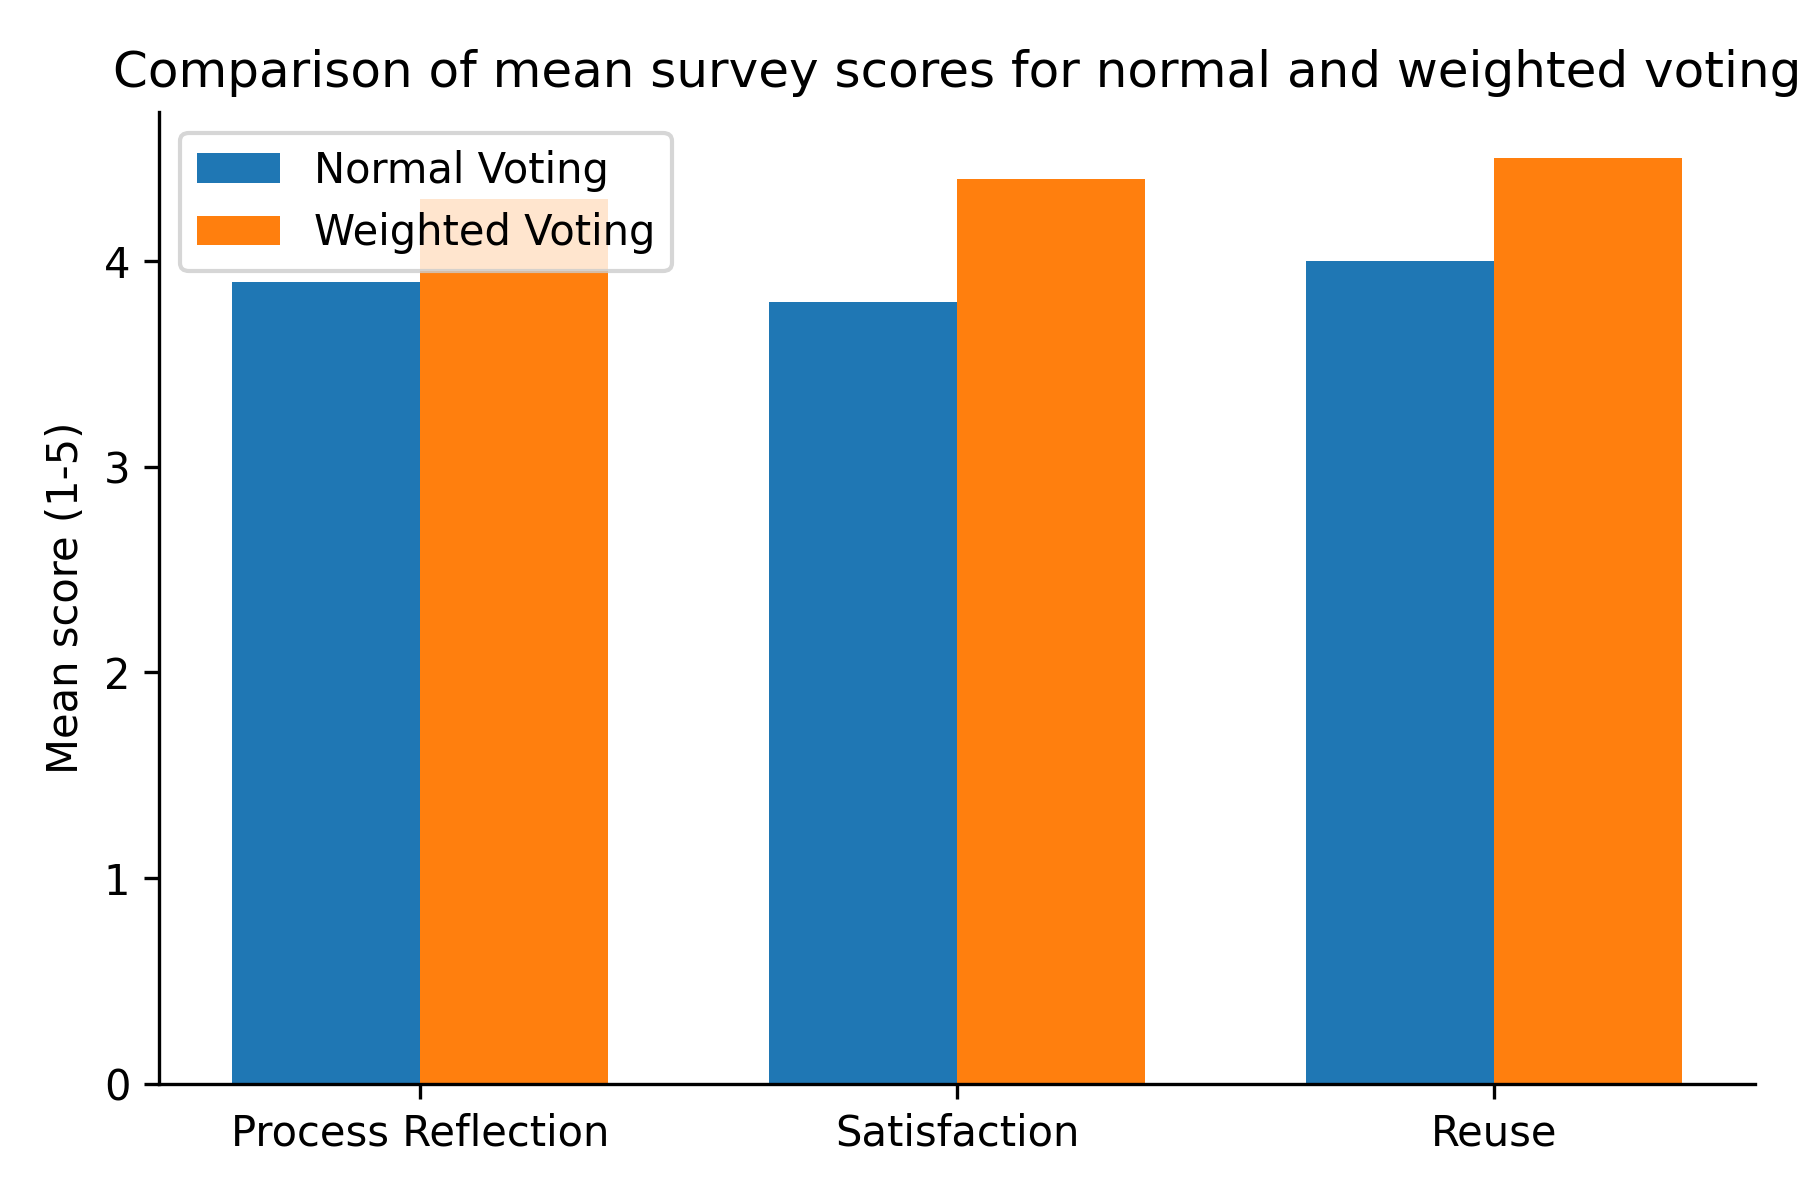
\includegraphics[width=0.8\linewidth]{imgs/token_comparison_chart.png}
    \caption{Comparison of mean survey ratings between plurality and weighted voting.  }
    \label{fig:bar-comparison}
\end{figure}

Taken together, these results indicate that allowing participants to allocate tokens not only changed one component of the ``Day~Out'' plan but also improved perceptions of fairness and satisfaction.  Participants overwhelmingly preferred the weighted method for future decisions, even while noting that the token interface could be refined.  The next chapter interprets these findings in relation to the broader literature on social choice and PD.
\doublespacing % Do not change - required

\chapter{Discussion}
\label{ch:discussion}

%%%%%%%%%%%%%%%%%%%%%%%%%%%%%%%%%%%%%%%
% IMPORTANT
\begin{spacing}{1} %THESE FOUR
\minitoc % LINES MUST APPEAR IN
\end{spacing} % EVERY
\thesisspacing % CHAPTER
% COPY THEM IN ANY NEW CHAPTER
%%%%%%%%%%%%%%%%%%%%%%%%%%%%%%%%%%%%%%%

% This chapter has been migrated from the original Chapter~5 and renumbered.
% It interprets the experimental results, situates them within the broader
% literature and assesses the strengths and limitations of the governance
% bot.  All references to earlier chapters have been updated to reflect the
% new chapter numbering.

This chapter interprets the experimental results, situates them within the
broader literature and assesses the strengths and limitations of the
governance bot.  We also discuss how the system relates to fundamental
concepts in social choice theory and PD.

\section{Interpretation of Results}

The experiment presented in Chapter~\ref{ch:experiments} yielded a rich set of quantitative and qualitative data.  Overall, the weighted token method was perceived as fairer and more satisfying than the standard plurality vote, and participants expressed a clear preference for using it in future decisions.  The following subsections interpret these findings and relate them to the broader literature.

\subsection*{Satisfaction and Fairness}
Across the three core post‑survey items—whether the process reflected the group’s preferences, satisfaction with the outcome and willingness to reuse the method—the weighted condition outperformed the plurality vote (Table~\ref{tab:survey-results}).  The mean differences were around half a point on a five‑point scale.  These results align with theoretical arguments that cardinal mechanisms allow participants to communicate the intensity of their preferences and can therefore produce outcomes that feel more legitimate to those with strong stakes \cite{Okasha2011}.  In our study the difference manifested most clearly in perceptions of fairness: the token‑allocation mechanism enabled participants to weight alternatives according to how much they cared about them, which translated into higher agreement that the outcome reflected the group’s will.  This echoes recent proposals for quadratic and staked voting in blockchain communities, where cardinal inputs are seen as a way to mitigate tyranny of the majority.  At the same time, the effect size was modest and only one component of the collective plan differed between the two conditions, suggesting that expressive mechanisms may primarily affect perceptions rather than radically altering outcomes in low‑stakes settings.

\subsection*{Ease of Use versus Expressiveness}
One potential drawback of weighted voting is increased cognitive load: participants must distribute a finite budget across multiple categories and options.  Our results indicate that this complexity was manageable.  Nine out of ten participants agreed or strongly agreed that the weighted process made them feel their voice was heard more clearly than in the plurality vote, and eight felt that they were able to use their tokens effectively.  Moreover, five agreed and four strongly agreed that thinking about token allocation made them consider their choices more carefully.  These findings suggest that the additional expressive power did not deter users; instead, it encouraged reflection.  Nevertheless, some participants requested clearer instructions and a more intuitive interface for token allocation.  In line with literature on PD \cite{Schuler1993PD}, ensuring that users understand the mechanics of a system is crucial for perceived fairness; future iterations should refine the token UI to reduce ambiguity.

\subsection*{Impact on Collective Decisions}
Despite the higher ratings for weighted voting, the two methods produced almost identical ``Day~Out'' plans.  The sole difference was the afternoon activity: the plurality vote selected sports, whereas the token mechanism selected visiting a museum or gallery.  This divergence illustrates how cardinal preferences can tip the balance when preferences are diverse but not strongly polarised.  Participants who cared deeply about a particular option could convey this by investing more tokens, thereby influencing the outcome even when they were a minority in the plurality vote.  In all other categories the same alternatives won under both rules, implying broad consensus.  These findings underscore that expressive mechanisms may have subtle but meaningful effects on collective decisions, especially when preferences vary in intensity but are not sharply divided.

\subsection*{Method Preference and Adoption}
When asked which mechanism they would choose for future group decisions, seven participants selected weighted voting outright and three selected weighted voting conditional on increased familiarity; none preferred the plurality rule.  Combined with the improvement in self‑reported understanding of voting methods (eight participants felt their knowledge improved), this suggests a strong appetite for more expressive decision tools.  Participants appeared willing to tolerate slight increases in complexity in exchange for feeling that their preferences were captured more faithfully.  This mirrors findings from studies of participatory budgeting and deliberative polling, where participants value being heard even when processes are more involved \cite{Talpin2011PB}.  Widespread adoption would nevertheless require user education and interface refinements to ensure newcomers can participate without confusion.

Qualitative feedback reinforced these interpretations.  Participants praised the overall concept and ease of use, while a minority requested clearer token allocation instructions.  No one criticised the mechanism itself, indicating general acceptance.  Together, the data show that weighted voting can enhance subjective fairness and satisfaction while remaining accessible, provided the interface communicates its mechanics effectively.

\section{Strengths and Limitations}

\textbf{Strengths}.  The primary strength of the project is its modular
architecture, which supports multiple classic voting mechanisms and can be
extended to include new rules.  Implementing the system on a popular
platform like Discord demonstrates the practicality of computational social
choice in real‑world settings.  The empirical evaluation combined pre‑ and
post‑survey data with objective log data, demonstrating the feasibility of
running controlled studies on a live messaging platform.  Using
standardised instruments and a counterbalanced design enabled meaningful
within‑subject comparisons across voting schemes and provided quantitative
evidence that weighted voting can improve perceptions of fairness and
satisfaction.

\textbf{Limitations}.  The participant pool was relatively small and
homogeneous—ten volunteers recruited from the researchers’ networks—which
limits the generalisability of the findings.  The \emph{Day~Out} scenario
was low‑stakes; responses may differ for more consequential decisions.
Discord’s interface constraints required custom solutions that may not
scale to a large number of options or users, and several participants
asked for clearer token‑allocation instructions.  The weighted mechanism
assumes that participants understand and interpret tokens as intended;
misunderstandings could lead to misrepresentations of preferences.  The
study did not compare the bot with other governance tools, which would
help contextualise its usability and effectiveness.  Future work should
address these limitations through larger and more diverse studies,
higher‑stakes scenarios, improved UI and comparative
evaluations.

\section{Relationship to Social Choice Theory}

The governance bot implements several classical social choice mechanisms.
Plurality and Borda count are positional scoring rules; approval voting
allows voters to endorse multiple alternatives; runoff and Condorcet methods
seek an alternative that would win in pairwise comparisons.  Weighted
voting introduces cardinal preferences reminiscent of quadratic voting
schemes.  Arrow’s impossibility theorem reminds us that no single rule
simultaneously satisfies all fairness axioms \cite{Arrow1951}; by allowing
communities to select among multiple mechanisms, the bot reflects the
engage–envision–enact philosophy and empowers participants to experiment
with the trade‑offs inherent in social choice.  The empirical results show
that allowing participants to allocate tokens increased perceived fairness
and satisfaction relative to the plurality rule.  This finding resonates
with Okasha’s observation that different evaluative virtues matter to
different participants \cite{Okasha2011} and supports arguments for
cardinal mechanisms.  At the same time, because only one category’s
outcome changed, the experiment illustrates that expressive methods may not
drastically alter group decisions in low‑stakes contexts.  Nevertheless, by
providing a concrete deployment of both ordinal and cardinal rules on a
messaging platform, the study contributes empirical evidence to debates
about cardinal versus ordinal preference aggregation.

The system also operationalises participatory and power‑sensitive design
principles.  By enabling users to propose rules, choose mechanisms and
withdraw consent, the bot provides meaningful control and transparency.
Nevertheless, there remain power dynamics inherent in digital platforms; as
Mertzani and Pitt caution, hybrid human–AI systems can reinforce
inequalities if those affected are not actively involved in design and
governance \cite{Mertzani2025SGML}.  Future work should explore how
machine‑learning tools, such as \emph{what‑if} predictors, can aid
communities without disempowering them.
\doublespacing % Do not change - required

\chapter{Reflections}
\label{chLast}

%%%%%%%%%%%%%%%%%%%%%%%%%%%%%%%%%%%%%%%
% IMPORTANT
\begin{spacing}{1} %THESE FOUR
\minitoc % LINES MUST APPEAR IN
\end{spacing} % EVERY
\thesisspacing % CHAPTER
% COPY THEM IN ANY NEW CHAPTER
%%%%%%%%%%%%%%%%%%%%%%%%%%%%%%%%%%%%%%%

% This chapter has been migrated from the original LastChapter and
% renumbered.  It provides a reflective assessment of the project from
% legal, ethical, environmental and inclusion perspectives, discusses
% quality management practices and introduces a new section on project
% limitations and technical challenges.

This final substantive chapter provides a reflective assessment of the
project from legal, ethical, environmental and inclusivity perspectives.
It also discusses quality management practices employed during
development.  Such reflections are required by the programme’s learning
outcomes and ensure that engineering work is situated within its broader
social context.

\section{Legal and Ethical Matters}

\textbf{Legal considerations}.  The governance bot processes user input on
Discord servers.  Although the bot stores only minimal metadata—such as
anonymised votes and tokens—it nevertheless interacts with personal data.
The implementation adheres to the spirit of data protection regulations
such as the UK GDPR.  No personally identifiable information is stored;
user identifiers are hashed before being persisted, and only aggregate
statistics are published.  Users are informed about how their data will
be used, and participation in weighted campaigns is strictly opt‑in.
Intellectual property rights were respected: external libraries were used
under appropriate licences, and contributions to the open‑source
repository are attributed.

The system implements privacy by design.  Each user’s unique Discord identifier
is passed through a cryptographic one‑way hash function before being
stored, and the original identifier is never written to the database.
The bot stores token allocations only in aggregated form; individual
allocations are deleted once the result has been announced.
Participation in weighted campaigns is explicitly opt‑in and users can
withdraw their consent at any time, upon which their votes and token
allocations are removed from the data store.  These practices align
with data‑protection principles of minimisation, purpose limitation
and the right to be forgotten.

\textbf{Ethical considerations}.  Algorithmic governance systems can
embed biases that disadvantage certain users.  To mitigate this, the bot
offers multiple voting mechanisms and allows communities to choose their
preferred method.  Weighted voting raises ethical questions about
commodifying preferences.  Tokens were framed as a budget for expressing
intensity rather than as a currency; no real financial stakes are
involved.  The experimental protocol received informal ethical approval
from the supervisor, and participants provided informed consent.  The
results were anonymised, and participants could withdraw at any time.

When designing the token system we avoided analogies that could be
interpreted as monetising influence.  Tokens are allocated equally to
all participants and cannot be purchased, transferred or saved across
decisions.  The budget of one hundred tokens provides sufficient
granularity to express intensity without overwhelming users; future
studies could experiment with different budgets.  Instructions
emphasise that tokens signify the strength of preference rather than
financial value, and the UI prevents over‑investment by
enforcing the budget constraint.  These choices are intended to
preserve the normative distinction between civic participation and
market exchange.

Beyond compliance with data protection statutes, algorithmic governance
raises broader questions of legitimacy and power.  The
Engage–Envision–Enact framework reminds us that democracy should not
be assumed to be a universal end state and that legitimacy derives from
meaningful, informed and revocable participation.  Designers must
therefore ensure that participants understand the voting mechanisms and
have the ability to contest outcomes or propose alternatives.  The
socially‑guided machine learning literature warns of the dangers of
``techno‑feudalism'' if AI systems mediate decisions without proper
oversight \cite{Mertzani2025SGML}.  While our bot does not employ
machine learning, future extensions (such as the proposed
\emph{what‑if} predictor) must be scrutinised for potential biases and
their impact on power relations within the community.

\section{Environmental and Social Impact}

\textbf{Environmental impact}.  The bot runs on modest cloud hardware
and uses lightweight data storage.  Energy consumption is minimal
compared with compute‑heavy AI systems.  The project’s main environmental
contribution lies in its potential to support collaborative decision‑making
that could, for example, promote sustainable activities (e.g., choosing a
low‑carbon outing) or facilitate coordination of community projects.  The
source code and documentation are released under an open‑source licence,
enabling reuse and reducing duplication of effort.

\textbf{Social impact}.  By empowering communities to participate in
governance, the bot can foster a sense of ownership and collective
responsibility.  However, digital divides persist: not all community
members have equal access to or familiarity with Discord.  To mitigate
exclusion, future versions could integrate with alternative platforms or
provide offline participation modes.  There is also a risk that weighted
voting may privilege vocal or well‑resourced participants if not carefully
explained.  Transparent rules and community moderation are essential to
prevent misuse.

Digital divides manifest along multiple dimensions: access to devices and
internet connectivity, familiarity with online platforms and ability to
navigate UIs.  To address these issues, future iterations of
the governance tool should implement cross‑platform clients—for example,
a web portal accessible via browsers, SMS‑based interfaces for users
without smartphones or dedicated mobile applications with offline
support.  Providing multilingual options and clear tutorials will help
broaden participation.  The token system must be accompanied by
transparent explanations and community guidelines to avoid perceptions
that influence is being bought.  Community moderation and participatory
rule‑setting processes can help ensure that weighting schemes are
understood and accepted.

Self‑organising decision systems must also guard against Goodhart’s
law: optimising for a single metric (for example, participation rate
or energy use) can distort behaviour and undermine the ultimate goals of
fairness or sustainability.  Implementing multiple measures and
qualitative feedback channels can help maintain balanced evaluation
criteria.

\section{Equality, Diversity and Inclusion}

The design sought to be inclusive of users with diverse abilities and
backgrounds.  Buttons and modal interfaces were labelled clearly, and
instructions avoided jargon.  Surveys asked participants about ease of
use to identify accessibility issues.  Weighted voting allows
individuals to distribute preference intensity, which can benefit
minorities by signalling strong support for less popular options.
Nonetheless, weighted schemes could disadvantage users unfamiliar with
token allocations.  Future work should include accessibility testing
with users from varied age groups, technical proficiencies and
disabilities.  Features such as screen‑reader compatibility, high‑contrast
colour schemes, keyboard navigation, descriptive alternative text for
icons and clear error prompts are essential to ensure that the bot is
usable by people with visual or motor impairments.  Providing input
methods beyond buttons—such as slash commands or voice interfaces—can
accommodate different interaction preferences.

Ensuring inclusivity also involves linguistic and cultural
considerations.  Many online communities span multiple countries and
language groups; therefore, future versions of the bot should support
multilingual interfaces and consider cultural differences in voting
norms.  Integration with platforms beyond Discord—including web portals
that work with screen readers, SMS‑based interfaces for users without
smartphones and printed ballots for in‑person meetings—could broaden
participation and bridge digital divides.  Engagement with community
stakeholders from the earliest design stages will help surface diverse
needs and avoid assumptions about homogeneity.  Co‑design workshops and
iterative user testing can ensure that the governance tool remains
accessible, equitable and culturally sensitive.

\section{Quality Management Systems}

Quality management was integral throughout the project.  The GitHub
repository used version control to track changes, with meaningful commit
messages explaining the rationale for modifications.  Continuous
integration scripts automatically ran unit tests on key functions, such as
proposal creation and vote counting, to detect regressions.  Code was
organised into modules with clear interfaces to facilitate peer review and
future maintenance.  Documentation was maintained in README files and
inline comments.  During deployment, logging and error handling were
implemented to monitor runtime behaviour and diagnose issues quickly.

Regular peer review sessions were held to inspect code for clarity,
conformance to style guidelines and potential security issues.  Issues
were tracked using GitHub’s issue tracker, and each feature branch
underwent automated testing and manual review before merging.  The use
of continuous integration ensured that refactoring or adding new voting
rules did not break existing functionality.  These practices align with
industry standards and facilitate future maintenance and collaboration.

\section{Project Limitations and Technical Challenges}

The design and implementation of the governance bot were subject to
several practical limitations and technical challenges.  First, the
Discord platform provides only a handful of interaction widgets: at most
five buttons per message, short text inputs in modals and no native
drag‑and‑drop or dropdown selectors.  Implementing complex voting rules
within these constraints required creative solutions.  For instance,
ranking alternatives for the Borda, IRV and Condorcet methods was
realised through a sequence of prompts asking users to select their next
preferred alternative rather than through a single ranked form.  Token
allocation in weighted voting involved increment and decrement buttons and
a progress bar to convey the remaining budget.  These sequential
interactions increase the number of clicks compared with native polls and
may introduce fatigue; however, they were necessary to comply with the
platform’s API limitations.

Second, the absence of real-time feedback mechanisms on Discord limited
the ability to provide immediate visualisations of current vote tallies.
To mitigate bandwagon effects—a phenomenon where voters are swayed by
interim results—the bot deliberately suppresses interim counts until
voting closes.  This design choice is grounded in the literature on the
bandwagon effect and aims to preserve independence of irrelevant
alternatives.  Nevertheless, it means that participants do not receive
dynamic feedback on how their community is voting, which may reduce
engagement for users accustomed to live polls.

Third, computational efficiency informed the choice of voting rules.  Some
systems in social choice, such as Kemeny’s method, are NP-hard to compute
exactly.  Our implementation therefore supports only polynomial-time
algorithms such as plurality, Borda, approval, instant runoff and
Condorcet (with a simple majority matrix).  While this decision aligns
with feasibility constraints, it excludes methods that satisfy stronger
fairness axioms but incur intractable computation.  Future work could
explore approximate algorithms or off-chain computation to expand the
available mechanisms.

Finally, developing a robust and secure bot requires careful handling of
concurrency and data persistence.  The event-driven nature of
\texttt{discord.py} demands asynchronous programming; mismanaging
coroutines can lead to deadlocks or lost updates.  Similarly, ensuring
that the database is updated atomically and that race conditions do not
corrupt state was a key challenge.  Logging, extensive testing and
incremental deployment helped address these issues but required
substantial engineering effort.  Recognising these limitations and
challenges provides valuable lessons for future iterations of the
governance platform.

% You can change the title of the conclusions by changing the text between { }
\conclusions{Conclusions and future directions} % Do not remove - required
% EDIT THE CONTENT OF THE FILE
% Conclusions.tex
% You can find it under the folder 
% "chapters" on the left column

% APPENDICES ARE OPTIONAL
% COMMENT OUT BOTH LINES BELOW TO REMOVE THEM
% ADD CHAPTERS TO ADD MULTIPLE APPENDICES
\appendix 
\doublespacing % Do not change - required

\chapter{Supplementary Materials}
\label{appendix}

\thesisspacing % Do not change - required

This appendix provides supplementary details to support the main text.

\section{Pre‑Voting Survey}
\label{appendix:pre-survey}

The pre‑voting survey gathers baseline information about participants’
experience with Discord, their familiarity with voting methods and their
attitudes towards fairness, speed and trust in decision procedures.  Unless
otherwise indicated, items are rated on a five‑point scale where higher
values indicate stronger agreement.

\begin{enumerate}
    \item \textbf{Consent to participate}.  Participants indicate whether they
    consent to participate in the study (Yes/No).
    \item \textbf{Name}.  Participants provide their name to match pre‑ and
    post‑responses.  Names will be anonymised during analysis.
    \item \textbf{Discord usage}.  ``Have you used Discord before?'' (Yes/No).
    \item \textbf{Group discussion frequency}.  ``How often do you
    participate in group discussions?'' (Always, Often, Sometimes, Rarely,
    Never).
    \item \textbf{Knowledge of plurality voting}.  ``Have you heard of
    plurality voting?'' (Yes/No).
    \item \textbf{Knowledge of weighted voting}.  ``Have you heard of
    weighted voting?'' (Yes/No).
    \item \textbf{Fairness importance}.  ``I care that the decision feels
    fair to the group.'' (1–5).
    \item \textbf{Speed vs fairness}.  ``I care more about speed than
    perfect fairness.'' (1–5).
    \item \textbf{Comfort with Discord polls}.  ``I’m comfortable using
    Discord polls for decisions.'' (1–5).
    \item \textbf{Openness to new methods}.  ``I’m open to trying different
    voting methods.'' (1–5).
    \item \textbf{Trust in explanation}.  ``I trust results more when the
    method is explained clearly.'' (Strongly disagree, Disagree, Neutral,
    Agree, Strongly agree).
    \item \textbf{Discord server confirmation}.  Participants confirm that
    they have joined the study’s Discord server (Yes).
\end{enumerate}

\section{Post‑Voting Survey}
\label{appendix:post-survey}

The post‑voting survey is administered after participants complete both
voting sessions.  It measures changes in understanding, satisfaction with
outcomes and perceptions of fairness and legitimacy for each method, as
well as experiences with token allocation and preferences for future
voting methods.

\subsection*{Change in understanding}
\begin{itemize}
    \item ``Compared to before, my understanding of voting methods is
    now …'' with response options: Much better, Better, Same, Worse,
    Much worse.
\end{itemize}

\subsection*{Outcome satisfaction for normal voting}
Participants rate each aspect of the final plan from 1 (Very poor) to
5 (Excellent) for the outcome produced by the normal voting session:
\begin{itemize}
    \item Breakfast.
    \item Transport.
    \item Hangout location.
    \item Lunch.
    \item Evening activity.
    \item Dinner.
\end{itemize}

\subsection*{Outcome satisfaction for weighted voting}
Participants provide analogous ratings for the outcome produced by the
weighted voting session:
\begin{itemize}
    \item Breakfast.
    \item Transport.
    \item Hangout location.
    \item Lunch.
    \item Evening activity.
    \item Dinner.
\end{itemize}

\subsection*{Outcome fairness and legitimacy for normal voting}
On a five‑point scale from Strongly disagree to Strongly agree, participants
indicate the extent to which:
\begin{itemize}
    \item The final decision felt fair.
    \item The process reflected group preferences.
    \item I would reuse this process in my groups.
    \item I feel satisfied with the outcome.
\end{itemize}

\subsection*{Outcome fairness and legitimacy for weighted voting}
Using the same scale as above, participants evaluate the weighted voting
outcome with respect to fairness, reflection of preferences, willingness to
reuse the process and satisfaction with the outcome.

\subsection*{Token allocation experience}
Participants respond to the following statements using a five‑point scale
from Strongly disagree to Strongly agree:
\begin{itemize}
    \item ``Thinking about the process of allocating tokens made me
    consider my choices more carefully.''
    \item ``I feel that I was able to use my tokens effectively.''
    \item ``The weighted voting process made me feel my voice was heard
    more clearly than in the normal vote.''
\end{itemize}
Participants are also asked whether their top choice on the main aspect
(e.g., the primary activity) won in each session (Yes, No, Close
second).

\subsection*{Preference for method}
Participants indicate which method they would prefer to use in the future
for a similar group decision, selecting one of the following options:
\begin{itemize}
    \item I would prefer normal voting.
    \item I would prefer weighted voting.
    \item I would prefer weighted voting, but only if I get more
    comfortable with it.
    \item I have no preference.
\end{itemize}

\subsection*{Discord poll usability}
Participants report whether the polls were easy to understand on Discord
(Yes, No, Could be improved).

\subsection*{Open feedback}
Participants are invited to provide one suggestion or comment to improve
the process in future iterations.  Responses to this open‑ended item will
be analysed qualitatively.


%\input{AppendixB.tex} % Example second appendix (need to create the file in "chapters")


\cleardoublepage % Do not change - required
\RemoveLabels % Do not change - required
\thesisspacing % Do not change - required
% \printbibliography[title={Bibliography},heading=bibintoc] % Do not change - required %i've commendted this out
\bibliographystyle{ieeetr}
\bibliography{references}
\end{document}
% I've added lines 149-152. Try compile with this once you've uploaded the file I sent via teams. 

\end{document}
